% Diese Datei ist Teil des Buchs "Schreibe Dein Programm!"
% Das Buch ist lizensiert unter der Creative-Commons-Lizenz
% "Namensnennung - Weitergabe unter gleichen Bedingungen 4.0 International (CC BY-SA 4.0)"
% https://creativecommons.org/licenses/by-sa/4.0/deed.de

\chapter{Videospiele programmieren}
\label{cha:representation-and-state}

In diesem Kapitel programmieren wir zum ersten Mal ein vollständiges,
benutzbares Programm, nämlich ein kleines Videospiel.  Dafür brauchen
wir zwei Zusätze für die Lehrsprache in DrRacket, die Teachpacks
\texttt{image.rkt} und \texttt{universe.rkt}.  Ersteres ist für das
Anzeigen der Grafik zuständig (wir haben es im ersten Kapitel schon
einmal benutzt), und \texttt{universe.rkt} ist dafür da, die Grafiken
zu bewegen und interaktiv zu machen.

FIXME: In diesem Kapitel programmieren wir ...

\section{Bilder mit \texttt{image.rkt}}

Für die Grafikprogrammierung mit \drscheme{} laden wir ein sogenanntes
\textit{Teachpack\index{Teachpack}}, ein kleiner Sprachzusatz, in
diesem Fall mit einer Reihe von Funktionen zur Erzeugung von Bildern.
Wir sind ihm bereits in Abschnitt~\ref{sec:rechnen-mit-bildern} auf
Seite~\pageref{sec:rechnen-mit-bildern} begegnet: Um das Teachpack zu
laden, musst Du im Menü \texttt{Sprache} (oder \texttt{Language} in
der englischen Ausgabe) den Punkt \texttt{Teachpack hinzufügen}
(\texttt{Add teachpack}) anwählen, und im dann erscheinenden
Auswahl-Dialog die Datei
\texttt{image.rkt\index{image.rkt@\texttt{image.rkt}}} auswählen.

Dieses Kapitel beschreibt die wichtigsten Funktionen des Teachpacks,
aber es gibt noch viel mehr davon.  Du kannst Dokumentation dazu
finden, indem Du in DrRacket im \texttt{Hilfe}- oder \texttt{Help}-Menü
auf die Racket-Dokumentation klickst, und dort nach
\texttt{2htdp/image} im Suchfeld eintippst.\footnote{Zum Zeitpunkt der
  Drucklegung leider nur auf Englisch.  Wir arbeiten an einer
  deutschen Übersetzung.}

\subsection{Einfache Bilder}

Im Teachpack \texttt{image.rkt} erzeugen verschiedene Funktionen
einfache Bilder.  So hat zum Beispiel die Funktion \texttt{rectangle}
folgende Signatur:\index{rectangle@\texttt{rectangle}}
% 
\begin{lstlisting}
(: rectangle (natural natural mode color -> image))
\end{lstlisting}
%
Dabei sind die ersten beiden Argumente Breite und Höhe eines Rechtecks
in Pixeln.
Das Argument mit Signatur \lstinline{mode}\index{mode@\texttt{mode}} ist eine Zeichenkette, die
entweder \lstinline{"solid"} oder \lstinline{"outline"} sein muss. Sie bestimmt,
ob das Rechteck als durchgängiger Klotz oder nur als Umriss gezeichnet
wird.  Das Argument mit der Signatur \lstinline{color}\index{color@\texttt{color}} ist eine
Zeichenkette, die eine Farbe (auf Englisch) bezeichnet, 
zum Beispiel \lstinline{"red"}, \lstinline{"blue"}, \lstinline{"yellow"},
\lstinline{"black"}, \lstinline{"white"} oder \lstinline{"gray"}.  Als Ergebnis
liefert \lstinline{rectangle} ein Bild, das von der \drscheme{}-REPL
entsprechend angezeigt wird wie andere Werte auch.  Beispiel:
%
\begin{lstlisting}
(rectangle 100 30 "outline" "brown")
|\evalsto| |
\includegraphics[scale=0.5]{i1world/rectangle}|
\end{lstlisting}
%
Es gibt es noch weitere Funktionen, die 
geometrische Figuren zeichnen:\index{circle@\texttt{circle}}
%
\begin{lstlisting}
(: circle (natural mode color -> image))
\end{lstlisting}
%
Die \lstinline{circle}-Funktion liefert einen Kreis, wobei das erste
Argument den Radius angibt.  Die \lstinline{mode}- und
\lstinline{color}-Argumente sind wie bei \lstinline{rectangle}.
Beispiel:
%
\begin{lstlisting}
(circle 50 "solid" "red")
|\evalsto| |
\includegraphics[scale=0.5]{i1world/circle}|
\end{lstlisting}
%
\begin{lstlisting}
(: ellipse (natural natural mode color -> image))
\end{lstlisting}
%
\index{ellipse@\texttt{ellipse}}Diese Funktion liefert eine Ellipse,
wobei das erste Argument die Breite und das zweite die Höhe angibt.
Beispiel:
%
\begin{lstlisting}
(ellipse 50 100 "solid" "green")
|\evalsto| |
\includegraphics[scale=0.5]{i1world/ellipse}|
\end{lstlisting}
%
\begin{lstlisting}
(: triangle (natural mode color -> image))
\end{lstlisting}
%
\index{triangle@\texttt{triangle}}Diese Funktion liefert ein nach oben
zeigendes gleichseitiges Dreieck, wobei das erste Argument die
Seitenlänge angibt.  Beispiel:
%
\begin{lstlisting}
(triangle 50 "solid" "gold")
|\evalsto| |
\includegraphics[scale=0.5]{i1world/triangle}|
\end{lstlisting}
%
\begin{lstlisting}
(: line (natural natural color -> image))
\end{lstlisting}
%
\index{line@\texttt{line}}zeichnet eine Linie.  Der Aufruf
\lstinline{(line $w$ $h$ $c$)} liefert ein Bild
mit Breite $w$ und Höhe $h$, in dem die Linie von der linken oberen in
die rechte untere Ecke verläuft.  Falls die Linie entlang der anderen
Diagonale verlaufen soll, kannst Du einfach das Vorzeichen von $w$
oder von $h$ umdrehen.  Beispiele:
%
\begin{lstlisting}
(line 150 100 "blue")
|\evalsto| |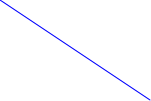
\includegraphics[scale=0.5]{i1world/line1}|
(line -150 100 "blue")
|\evalsto| |
\includegraphics[scale=0.5]{i1world/line2}|
\end{lstlisting}
%
Wir können auch ein Bild erzeugen, in dem Text steht, und zwar mit der
Funktion \lstinline{text}\index{text@\texttt{text}}, die folgende Signatur hat:
%
\begin{lstlisting}
(: text (string natural color -> image))
\end{lstlisting}
%
Die Zahl ist die Höhe der Buchstaben.  Beispiel:
%
\begin{lstlisting}
(text "Schreibe Dein Programm!" 20 "red")
|\evalsto| |
\includegraphics[scale=0.5]{i1world/text}|
\end{lstlisting}
%
Manchmal reichen einfache Rechtecke und Kreise nicht aus und wir
wollen komplexere Formen erzeugen.  Eine Möglichkeit ist die Funktion
\lstinline{polygon}\index{polygon@\texttt{polygon}}, die ein n-Eck
zeichnet.  Sie hat folgende Signatur:
%
\begin{lstlisting}
(: polygon ((list-of (mixed posn pulled-point)) mode color -> image)) 
\end{lstlisting}
%
Diese Funktion akzeptiert eine Liste von Eckpunkten und die üblichen
\lstinline{mode}- und \lstinline{color}-Argumente.  Ein Eckpunkt 
muss entweder zur Signatur \lstinline{posn} oder zu
\lstinline{pulled-point} gehören.  Das sind eingebaute Record-Typen,
bei denen \lstinline{posn}\index{posn@\texttt{posn}} so definiert sein könnte:
%
\begin{lstlisting}
(define-record posn
  make-posn
  posn?
  (posn-x real)
  (posn-y real))
\end{lstlisting}
%
Dieser Typ definiert also ganz normale kartesische Koordinaten mit X-
und Y-Komponente.  Hier ist ein Beispiel für ein Polygon mit solchen
Eckpunkten:
%
\begin{lstlisting}
(polygon (list (make-posn 0 0)
               (make-posn -20 40)
               (make-posn 120 0)
               (make-posn -20 -40))
         "solid"
         "plum")
|\evalsto| |
\includegraphics[scale=0.5]{i1world/polygon1}|
\end{lstlisting}
%
Bei \lstinline{posn}-Eckpunkten sind die Kanten also alles gerade
Linien.  Mit \lstinline{pulled-point}-Eckpunkten ist es möglich, die
Kanten zu Kurven zu machen.  Auch \lstinline{pulled-point} ist ein
Record-Typ, der so definiert sein könnte:
%
\begin{lstlisting}
(define-record pulled-point
 make-pulled-point
 pulled-point?
 (pulled-point-lpull real)
 (pulled-point-langle real)
 (pulled-point-x real)
 (pulled-point-y real)
 (pulled-point-rpull real)
 (pulled-point-rangle real))
\end{lstlisting}
%
Wie \lstinline{posn} hat auch \lstinline{pulled-point} eine X- und
eine Y-Koordinate.  Außerdem gibt es zwei "<Pull">- und zwei
"<Angle">-Komponenten, die spezifizieren, wie die Kanten gebogen
werden.  Abbildung~\ref{fig:pulled-point} zeigt, wie das
funktioniert:  Für jeden Eckpunkt gibt es eine Kante vom
vorigen Punkt~-- die \emph{eingehende} Kante~-- und die Kante zum nächsten
Punkt~-- die \emph{ausgehende} Kante.

\begin{figure}[tb]
  \centering
  \def\svgwidth{0.4\textwidth}
  \input{i1world/pulled-point.pdf_tex}
  \caption{Funktionsweise von \lstinline{pulled-point}}
  \label{fig:pulled-point}
\end{figure}
%
Die \lstinline{pulled-point-langle}-Komponente gibt den Winkel an, mit
dem die eingehende Kante gebogen wird, die
\lstinline{pulled-point-rangle}-Komponente den Winkel ist für die
ausgehende Kante zuständig.  Abbildung~\ref{fig:pulled-point} zeigt,
wie \lstinline{langle} und \lstinline{rangle} auf den Punkt mit der
Nummer~2 wirken: Die eingehende Kante kommt von Punkt~1 her, die
ausgehende Kante geht zu Punkt~3.  Die Komponenten
\lstinline{pulled-point-lpull} und \lstinline{pulled-point-rpull}
geben wann, wieviel die Kanten verbogen werden~-- das sind
typischerweise Zahlen zwischen 0 und 1.
%
\begin{lstlisting}
(polygon (list (make-pulled-point 1/2 0 0 0 1/2 -20)
                           (make-posn -20 40)
                           (make-pulled-point 1/2 -20 120 0 1/2 20)
                           (make-posn -20 -40))
                     "solid"
                     "plum")
|\evalsto| |
\includegraphics[scale=0.5]{i1world/polygon2}|
\end{lstlisting}
%
add-curve

\subsection{Bilder zusammensetzen und verändern}

Da diese geometrischen Formen für sich genommen langweilig sind, können
mehrere Bilder miteinander kombiniert werden.


Zum Aufeinanderlegen gibt es die Funktion \lstinline{overlay}\index{overlay@\texttt{overlay}}:
%
\begin{lstlisting}
(: overlay (image image h-place v-place -> image))
\end{lstlisting}
%
Dabei sind die ersten beiden Argumente die Bilder, die
aufeinandergelegt werden~-- das zweite auf das erste.
Die beiden anderen Argumente geben an, wie
die beiden Bilder zueinander positioniert werden.  Die Signatur
von \lstinline{h-place}, das die horizontale Positionierung festlegt,
ist:\index{h-place@\texttt{h-place}}
%
\begin{lstlisting}
(define h-place
   (signature
      (mixed natural
             (enum "left"
                   "right"
                   "center"))))
\end{lstlisting}
%
Im ersten Fall, wenn es sich um eine Zahl $x$ handelt, wird das zweite
Bild $x$ Pixel vom linken Rand auf das erste gelegt.  Die drei
Fälle mit Zeichenketten sagen, dass die Bilder am linken Rand beziehungsweise am
rechten Rand bündig plaziert werden, beziehungsweise das zweite Bild horizontal
in die Mitte des ersten gesetzt wird.
Dementsprechend ist
\lstinline{v-place}, das die vertikale Positionierung festlegt,
wie folgt definiert:\index{v-place@\texttt{v-place}}
%
\begin{lstlisting}
(define h-place
   (signature
      (mixed natural
             (enum "top"
                   "bottom"
                   "center"))))
\end{lstlisting}
%
Im ersten Fall, wenn es sich um eine Zahl $y$ handelt, wird das zweite
Bild $y$ Pixel vom oberen Rand auf das erste gelegt.  Die drei
Fälle mit Zeichenketten sagen, dass die Bilder am oberen Rand beziehungsweise am
unteren Rand bündig plaziert werden, beziehungsweise das zweite Bild vertikal
in die Mitte des ersten gesetzt wird.

Das Bild, das bei \lstinline{overlay} herauskommt, ist groß genug, dass
beide Eingabebilder genau hineinpassen.

overlay/xy

scale

place-image/align


Die folgenden Hilfsfunktionen sind Spezialfälle von \lstinline{overlay}:
%
\begin{lstlisting}
(: above  (image image h-mode -> image))
(: beside (image image v-mode -> image))
\end{lstlisting}
%
Die Funktion \lstinline{above}\index{above@\texttt{above}} ordnet zwei
Bilder übereinander an, \lstinline{beside}\index{beside@\texttt{beside}}
nebeneinenander.  Dabei ist \lstinline{h-mode} eine der Zeichenketten
\lstinline{"left"}, \lstinline{"right"} und \lstinline{"center"}, die angibt, ob die
Bilder bei \lstinline{above} an der linken oder rechten Kante oder der
Mitte ausgerichtet werden.  Entsprechend ist \lstinline{v-mode} eine der
Zeichenketten \lstinline{"top"}, \lstinline{"bottom"} und \lstinline{"center"}, die
angibt, ob die Bilder bei \lstinline{beside} oben, unten oder an der
Mitte ausgerichtet werden.

Die Funktionen \lstinline{clip} und \lstinline{pad} beschneiden beziehungsweise
erweitern ein Bild:\index{clip@\texttt{clip}}\index{pad@\texttt{pad}}
%
\begin{lstlisting}
(: clip (image natural natural natural natural -> image))
(: pad  (image natural natural natural natural -> image))
\end{lstlisting}
%
Ein Aufruf \lstinline{(clip $i$ $x$ $y$ $w$ $h$)} liefert 
das Teilrechteck des Bildes $i$ mit Ecke bei $(x, y)$, Breite $w$ und
Höhe $h$.  Der Aufruf \lstinline{(pad $i$ $l$ $r$ $t$ $b$)}
fügt an den Seiten von $i$ noch transparenten Leerraum an: $l$ Pixel
links, $r$ Pixel rechts, $t$ Pixel oben und $b$ Pixel unten.

Abbildung~\ref{fig:image-ss} zeigt, wie sich die einige der
\texttt{image.ss}-Funktionen in der \drscheme{}-REPL verhalten.

\begin{figure}
  \centering
  TBD
  \caption{Eingefügte Bilder in der \drscheme{}-REPL}
  \label{fig:image-insert}
\end{figure}
%
Es ist auch möglich, externe Bilder-Dateien in
\texttt{image.rkt}-Bilder zu verwandeln.  Dazu dient der Menüpunkt
\texttt{Bild einfügen} im \texttt{Spezial}-Menü:  \drscheme{} fragt nach dem
Namen einer Bilddatei, die dann in den Programmtext da eingefügt wird,
wo der Cursor steht.  Die eingefügten Bilder dienen dann als
Literale für Bild-Objekte.  Abbildung~\ref{fig:image-insert} zeigt ein
Beispiel.

Die folgenden Funktionen ermitteln Breite und Höhe
eines Bildes:\index{image-width@\texttt{image-width}}\index{image-height@\texttt{image-height}}
%
\begin{lstlisting}
(: image-width  (image -> natural))
(: image-height (image -> natural))
\end{lstlisting}


\section{Modelle und Ansichten}


TBD

\section{Bewegung und Zustand}

TBD  Dafür ist ein weiteres Teachpack namens
\texttt{universe.ss}\index{universe.ss@\texttt{universe.ss}} zuständig.  Es
kann in \drscheme{} genauso wie bei \texttt{image.rkt}
geladen werden.  

Alle Definitionen von
\texttt{image.rkt} sind auch in \texttt{universe.ss} verfügbar.

In der Terminologie von \texttt{universe.ss} ist ein Modell eine
\textit{world}, auf deutsch eine \textit{Welt}: Die Idee dahinter
ist, dass ein Bild eine Ansicht einer kleinen Welt ist.  Damit das
funktioniert, muss bei \texttt{universe.ss} eine erste Welt angemeldet
werden, zusammen mit Angaben, wie groß die Ansicht wird.  Dazu gibt es
die Funktion \texttt{big-bang}\index{big-bang@\texttt{big-bang}}:
%
\begin{lstlisting}
(: big-bang (natural natural number world -> #t))
\end{lstlisting}
%
("<Big Bang"> heißt zu deutsch "<Urknall">.)
Die ersten beiden Argumente geben Breite und Höhe der Ansicht an.  Das
dritte Argument gibt die Dauer (in Sekunden) zwischen Ticks der Uhr
an, die für die Animation benötigt wird.  Das vierte Argument gibt
schließlich die erste Welt an.  (Der Rückgabewert, immer
\lstinline{#t}, ist ohne Bedeutung.)  Für den Himmel mit
Sonne sieht der Aufruf von \texttt{big-bang} folgendermaßen aus:
%
\begin{lstlisting}
(big-bang sky-width sky-height 0.1 0)
\end{lstlisting}
%
Dieser Aufruf erzeugt ein Fenster mit Breite und Höhe des Himmels,
startet die Uhr, die jede Sekunde zehnmal tickt, und legt als erste
Welt "<0">, also den Anfang der Zeit fest.  (Eine zehntel Sekunde
reicht etwa aus, damit die Animation dem menschlichen Auge als
"<Bewegung"> erscheint.)

Damit das Teachpack die Welt in eine Ansicht umwandeln kann, muss eine
entsprechende Ansicht angemeldet werden.  Dafür ist die Funktion
\texttt{on-redraw\index{on-redraw@\texttt{on-redraw}}} zuständig:
%
\begin{lstlisting}
(: on-redraw ((world -> image) -> #t))
\end{lstlisting}
%
Als Argument akzeptiert \texttt{on-redraw} also eine Funktion, die aus
einer Welt ein Bild macht.  TBD

Auch diese Funktion muss noch beim Teachpack angemeldet werden.  Dafür
die Teachpack-Funktion
\texttt{on-tick-event\index{on-tick-event@\texttt{on-tick-event}}}
zuständig:
%
\begin{lstlisting}
(: on-tick-event ((world -> world) -> #t))
\end{lstlisting}
%
Die \texttt{on-tick-event}-Funktion akzeptiert eine Funktion, die bei
jedem Uhren-Tick aufgerufen wird, um aus der "<alten"> Welt eine neue
zu machen.  Auf diese Beschreibung und auch auf die Signatur
passt aber \texttt{next-time}.  Der Aufruf kann also so aussehen:
%
\begin{lstlisting}
(on-tick-event next-time)
\end{lstlisting}
%
Wenn das Programm
beendet werden soll, muss \texttt{on-tick-event} die Funktion
\texttt{end-of-time\index{end-of-time@\texttt{end-of-time}}} des
Teachpacks aufrufen, die folgende Signatur hat:
%
\begin{lstlisting}
(: end-of-time (string -> world))
\end{lstlisting}
%

\section{Andere Welten}

Eine kleine (wenn auch nicht besonders sinnvolle) Erweiterung zeigt,
wie die Animation auf Benutzereingaben reagieren kann.  Dazu muss sie
noch eine weitere Funktion anmelden, und zwar mittels
\texttt{on-key-event\index{on-key-event@\texttt{on-key-event}}}, das
ähnlich funktioniert wie \texttt{on-tick-event}:
%
\begin{lstlisting}
(: on-key-event ((world string -> world) -> #t))
\end{lstlisting}
%
Die Funktion, die mit \texttt{on-key-event} angemeldet wird, wird
immer aufgerufen, wenn der Benutzer eine Taste drückt.  Welche Taste
gedrückt wurde, gibt das zweite Argument 
an.  Wenn der Benutzer eine reguläre Zeichen-Taste drückt (also keine
Cursor-Taste o.ä.), ist dieses Argument eine Zeichenkette bestehend
aus diesem einen Zeichen.

TBD

\section*{Aufgaben}

TBD

\begin{aufgabe}
  Schreiben Sie ein kleines Telespiel Ihrer Wahl.
\end{aufgabe}

%%% Local Variables: 
%%% mode: latex
%%% TeX-master: "i1"
%%% End: 

